\documentclass[a4paper]{article}
\usepackage[affil-it]{authblk}
\usepackage[english]{babel}
\usepackage[backend=bibtex,style=numeric]{biblatex}

\usepackage{geometry}
\geometry{margin=1.5cm, vmargin={0pt,1cm}}
\setlength{\topmargin}{-1cm}
\setlength{\paperheight}{29.7cm}
\setlength{\textheight}{25.3cm}

% useful packages.
\usepackage{amsfonts}
\usepackage{amsmath}
\usepackage{amssymb}
\usepackage{amsthm}     
\usepackage{enumerate} %enumerate environment
\usepackage{graphicx}
\usepackage{multicol}
\usepackage{fancyhdr}
\usepackage{layout}
\usepackage{ctex}      %中文环境
\usepackage{booktabs}  %三线表
\usepackage{verbatim}  %comment environment
\usepackage{float}     %强制表格图片位置
\usepackage{listings}  %insert code in latex
\usepackage{fontspec}  %font support
\usepackage{tikz}
\usepackage{makecell}
\usetikzlibrary{intersections}
\usepackage{arydshln}
\usepackage{mathptmx}
\usepackage{helvet}
\usepackage{courier}
\usepackage[colorlinks,linkcolor=blue]{hyperref}
\usepackage{xcolor}
\definecolor{mygreen}{rgb}{0,0.6,0}
\definecolor{lightgrey}{rgb}{0.95,0.95,0.95}
\definecolor{winered}{rgb}{0.5,0,0}
\definecolor{mymauve}{rgb}{0.58,0,0.82}
\lstset{
      backgroundcolor=\color{lightgrey},
      basicstyle             = \ttfamily,
      breakatwhitespace      = false,
      breaklines             = true,
      captionpos             = none,
      commentstyle           = \color{mygreen}\bfseries,
      extendedchars          = false,
      keepspaces             = true,
      keywordstyle           = \color{winered},         % keyword style
      language               = C++,                     % the language of code
      otherkeywords          = {string},
      numberstyle            = \tiny\color{mygray},
      rulecolor              = \color{black},
      showspaces             = false,
      showstringspaces       = false,
      showtabs               = false,
      stepnumber             = 1,
      stringstyle            = \color{mymauve},         % string literal style
      tabsize                = 2,
      title                  = \lstname,
      aboveskip              = 0pt,
      belowskip              = 0pt,
      columns                = flexible
}

% some common command
\newcommand{\dif}{\mathrm{d}}
\newcommand{\avg}[1]{\left\langle #1 \right\rangle}
\newcommand{\norm}[1]{\left\| #1 \right\|}
\newcommand{\difFrac}[2]{\frac{\dif #1}{\dif #2}}
\newcommand{\pdfFrac}[2]{\frac{\partial #1}{\partial #2}}
\newcommand{\OFL}{\mathrm{OFL}}
\newcommand{\UFL}{\mathrm{UFL}}
\newcommand{\fl}{\mathrm{fl}}
\newcommand{\op}{\odot}
\newcommand{\Eabs}{E_{\mathrm{abs}}}
\newcommand{\Erel}{E_{\mathrm{rel}}}
\addbibresource{citation.bib}

\begin{document}
% =================================================
\title{Numerical Analysis chapter 1 programming report}

\author{Zhouyue Qian 3220104074
  \thanks{Electronic address: \texttt{3220104074@edu.zju.cn}}}
  \thanks{Translator for some paragraph\cite{kimiassistant}}
\affil{(Information and Computational Science Class 2201), Zhejiang University }


\date{Due time: \today}

\maketitle

\begin{abstract}
   This is the programming homework of chapter 1, which includes a equation solver. 
   I designed a base class for a solver, from which the bisection, Newton, and secant methods are derived. 
   This is specifically accomplished through overloading and inheritance.
\end{abstract}

\section*{A-Description}
The program is designed to solve the equation $f(x)=0$ using the bisection, Newton, and secant methods.
The base class abstracts the solution function and the destructor of the function.

\begin{lstlisting}
  class EquationSolver {
    public:
        virtual double solve() = 0 ;
        virtual ~EquationSolver() = default;
};
\end{lstlisting}
As for the three specific methods, they are directly inherited from the base class, and the functions use C++ pointers.\cite{deepseek}
\begin{lstlisting}
  double (*f)(double); //函数
  double (*df)(double); //一阶导数
\end{lstlisting}

\section*{B}
After the program is run, the following results are obtained:
\begin{figure}[H]
  \centering
  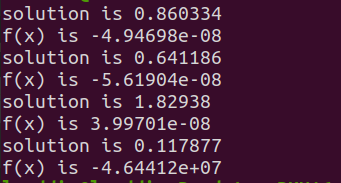
\includegraphics[width=0.8\textwidth]{B_result.png}
  \caption{results of B}
\end{figure}
We could find that the errors of the first three zero points are very small. Nevertheless, the error of the fourth zero point is relatively large.
The function values are very large. It is obvious that this zero point is not a real zero point.
So to find out why this happens, I have drawn the function graph.\cite{geogebra}
\begin{figure}[H]
  \centering
  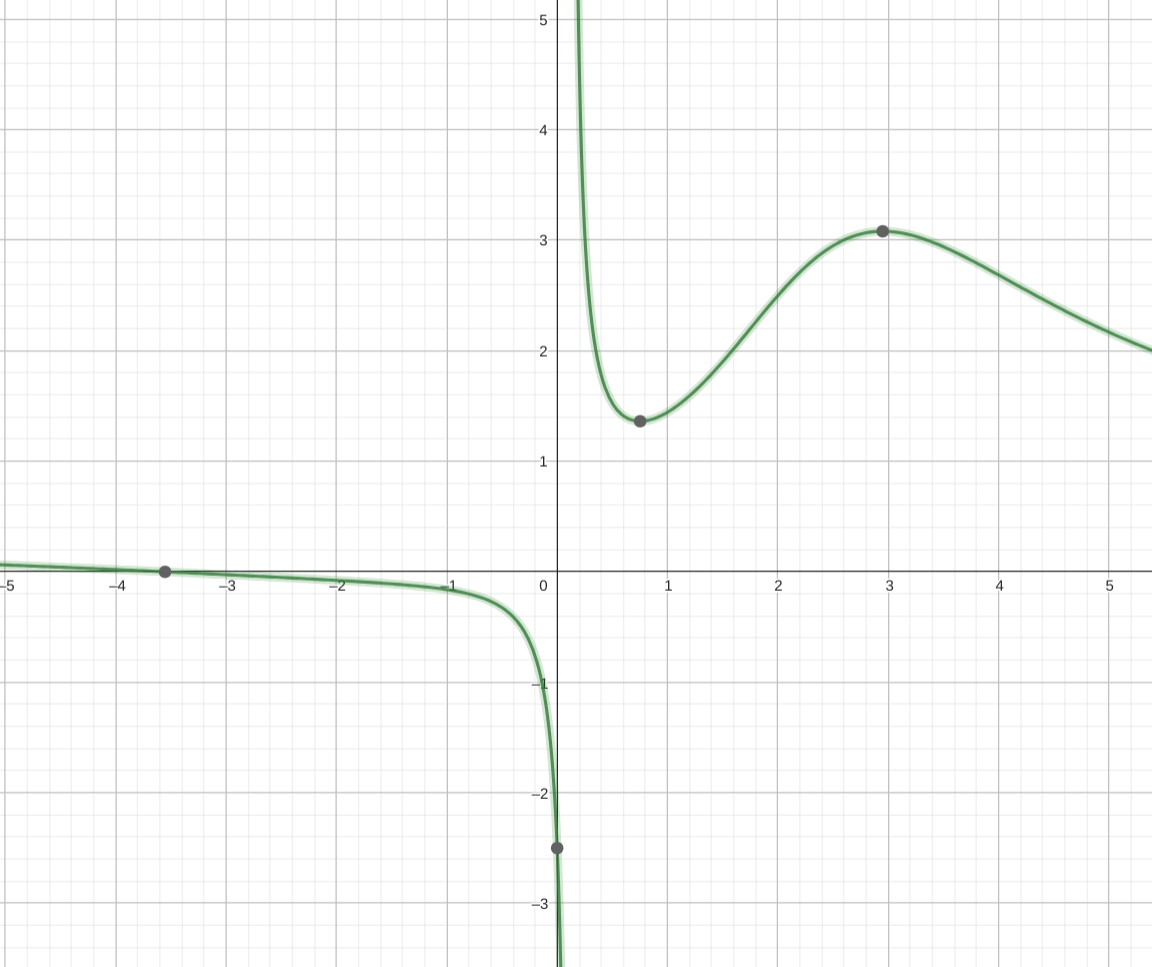
\includegraphics[width=0.8\textwidth]{B_4.jpeg}
  \caption{graph of function4}
\end{figure}
From the image, we can observe that the function is not continuous near $x = 0$. We designate this point of discontinuity as $\alpha$. 
Therefore, the data we ultimately obtain through the bisection method is the result of breaking out after the interval length becomes smaller than $\delta$, and this result approaches $\alpha$. 
Since the function does not meet the criteria for the bisection method, we cannot obtain the exact zero point.

\section*{C}
\begin{figure}[H]
  \centering
  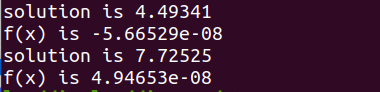
\includegraphics[width=0.8\textwidth]{C.png}
  \caption{results of C}
\end{figure}
We could find that the errors of the zero points are very small, which means we have already found the exact zero points.


\section*{D}
\begin{figure}[H]
  \centering
  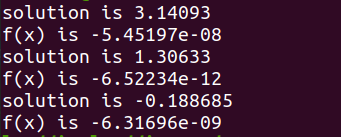
\includegraphics[width=0.8\textwidth]{D1.png}
  \caption{results of D}
\end{figure}
We could find that the errors of the zero points are very small, which means we have already found the exact zero points.
However, plotting the graph of the function, I find that these functions has many zero points.
\begin{figure}[H]
  \centering
  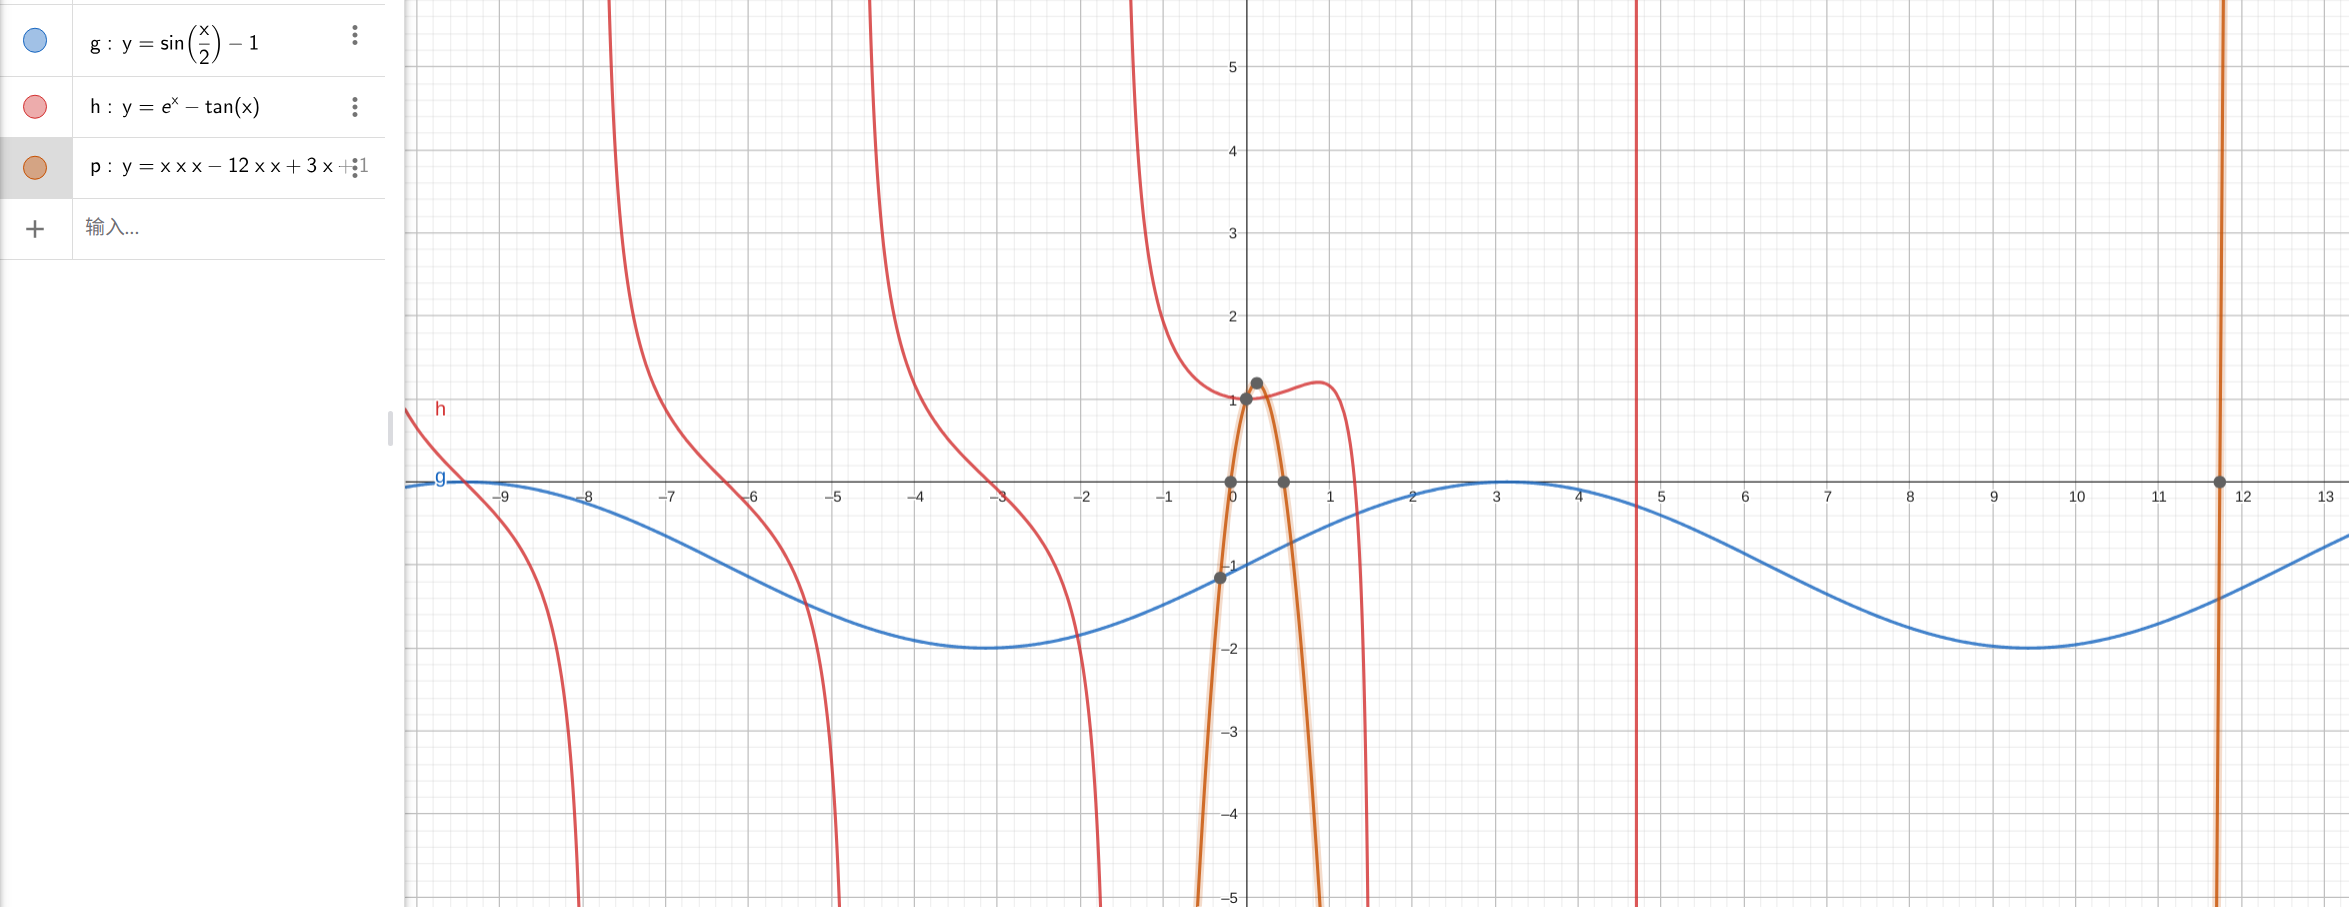
\includegraphics[width=0.8\textwidth]{D_f123.png}
  \caption{graph of function1}
\end{figure}
So, I change $x_0$ and $x_1$ to find different zero points.
\begin{table}
  \centering
  \begin{tabular}{|c|c|}
  \hline
  \textbf{$x_0$} & \textbf{$x_1$} \\ \hline
  $-3\pi$ & $-3.5\pi$ \\ \hline
  4 & 5 \\ \hline
  11& 12 \\ \hline
  \end{tabular}
\end{table}

\section*{E}
\begin{figure}
  \centering
  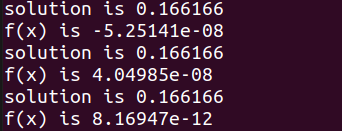
\includegraphics[width=0.8\textwidth]{E.png}
  \caption{results of E}
\end{figure}
We could find that the errors of $V$ are very small, which means we have already found the exact zero points.
This three zero point is generated by the three methods.

\section*{F}
\begin{figure}
  \centering
  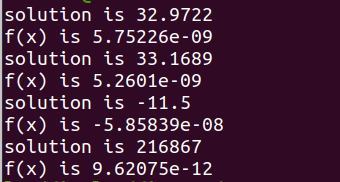
\includegraphics[width=0.8\textwidth]{F.png}
  \caption{results of F}
\end{figure}
\subsection*{a,b}
 The results have shown in the pics.

\subsection*{c}
We find that if we have totally different zero point in $a$. Below is the graph of the function.
\begin{figure}[H]
  \centering
  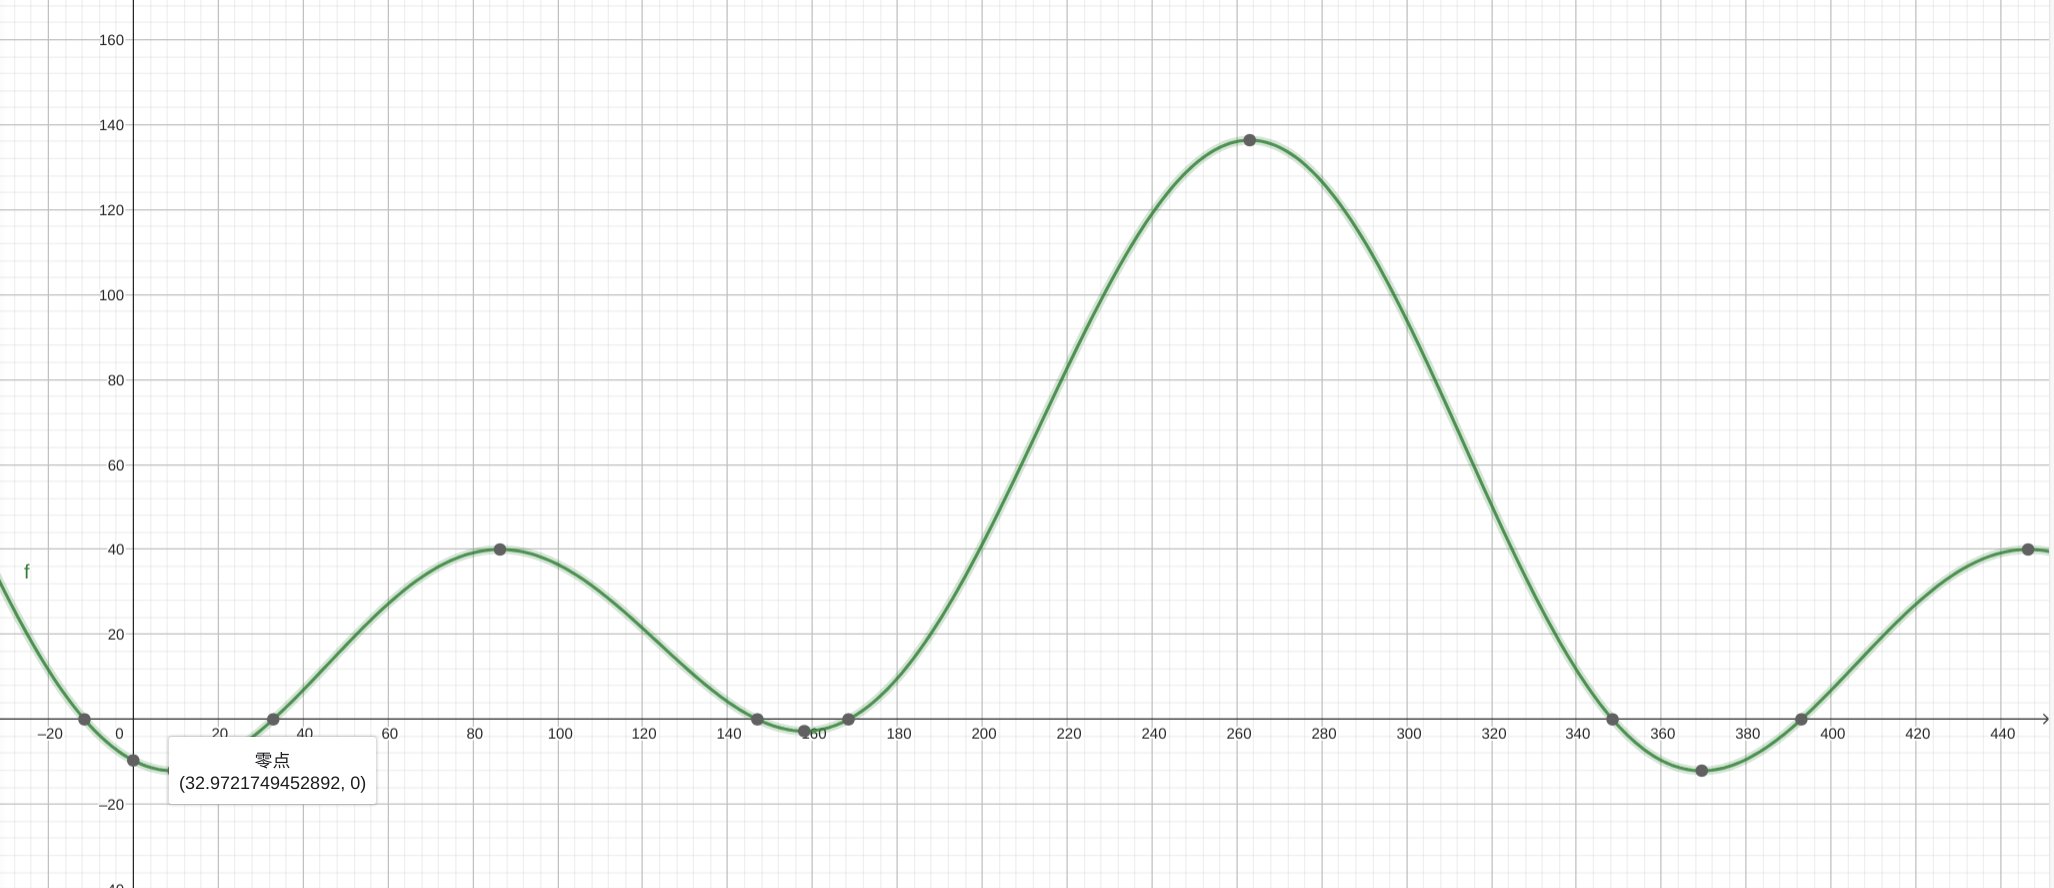
\includegraphics[width=0.8\textwidth]{F_f.png}
  \caption{graph of function}
\end{figure}\cite{geogebra}
From the graph, we could tell that $f(x)$ has tons of zero points. 
The function is monotonically increasing in the domain where x equals 33. Moreover, the function's concavity remains essentially unchanged.
\begin{itemize}
  \item if the initial value is taken near 0, since this part is monotonically decreasing and the concavity remains unchanged, it will iterate to a zero point on the left side of 0. 
  \item However, when taken near 90, due to the distance from the zero point being relatively far and the absolute value of the secant slope being very small, after continuous iteration, the zero point will eventually converge to another zero point that is farther away from the initial value.
\end{itemize}



% ===============================================
\section*{ \center{\normalsize {Acknowledgement}} }
\printbibliography

\end{document}

